
\section{Examples}

\textcolor{blue}{DG: The UCVM framework is comprised of multiple commands for data retrieval and graphical plotting. The sections below describe four of the most common utilities that are used within the framework.}

\subsection{The \textup{\texttt{ucvm\_query}} command}

Here is an example of how to run this command.

\begin{lstlisting}[
	frame=none,
	basewidth={0.45em,0.4em},
	basicstyle=\ttfamily\footnotesize,breaklines=true,
	linewidth=0.98\columnwidth,xleftmargin=0.07\columnwidth,
	numbers=left,numberblanklines=true,numberstyle=\scriptsize\color{mylistingnclr}]
> ./ucvm_query -f $UCVM_DIR/conf/ucvm.conf -m cvms
\end{lstlisting}

Note that the location of the package configuration file needs to be passed to the command using the flag ``\texttt{-f}'' and that the model to be used is set with the ``\texttt{-m}'' flag. 

\subsection{The \textup{\texttt{ucvm2mesh}} command}

This command generates a mesh or grid in either IJK-12, IJK-20, IJK-32, or SORD formats. The formats IJK-12, IJK-20, IJK-32, for instance, are used in discrete finite difference models for wave propagation simulations by the code \textcolor{red}{AWP-ODC (?) \citep{Cui_2010_Proc}}. SORD, on the other hand, is a format designed to interface with a finite element code used to simulate dynamic rupture processes (also called SORD) \citep{Ely_2009_GJI}. The \texttt{ucvm2mesh} takes as input a configuration file that is passed on as an argument using the flag ``\texttt{-f}''. This file specifies the model to be used, the region size, and the resolution of the mesh or grid. The following example shows how to execute this command.

\begin{lstlisting}[
	frame=none,
	basewidth={0.45em,0.4em},
	basicstyle=\ttfamily\footnotesize,breaklines=true,
	linewidth=0.98\columnwidth,xleftmargin=0.07\columnwidth,
	numbers=left,numberblanklines=true,numberstyle=\scriptsize\color{mylistingnclr}]
> ./ucvm2mesh -f ./ucvm2mesh_example.conf
\end{lstlisting}

\subsection{The \textup{\texttt{ucvm2etree}} command}

The command \texttt{ucvm2etree} builds a materialized model in the form of an etree database, which uses an octree unstructured mesh-like format that adjust octant sizes to a specific resolution based on the material properties in the CVM being used at every point in a given volume. Resulting etrees built using this command are stand-alone discrete representations of a given velocity mode, and can be used as input models for other operations using UCVM. They can also be queried separately using APIs distributed with the etree library. In wave propagation problems, etrees are used by the code Hercules \citep{Tu_2006_SC, Taborda_2010_Tech} in earthquake ground motion simulations. As in the previous case, this command takes an argument input configuration file. The following example shows how to execute this command.

\begin{lstlisting}[
	frame=none,
	basewidth={0.45em,0.4em},
	basicstyle=\ttfamily\footnotesize,breaklines=true,
	linewidth=0.98\columnwidth,xleftmargin=0.07\columnwidth,
	numbers=left,numberblanklines=true,numberstyle=\scriptsize\color{mylistingnclr}]
> ./ucvm2etree -f ./ucvm2etree_example.conf
\end{lstlisting}

Note that \texttt{ucvm2etree} is the serial version of other parallel (MPI) commands used to build large materialized models in high performance computer systems. Parallel tools for building etrees are useful because regional size simulations require models that can be on the order of hundreds of gigabytes to terabytes and can take significant time and resources to build. Thus, for large etrees, we strongly recommend using the \texttt{ucvm2etree-extract-MPI}, \texttt{ucvm2etree-sort-MPI}, and \texttt{ucvm2etree-merge-MPI} commands explained below.


\subsection{The \textup{\texttt{horizontal\_slice.py}} command}

\textcolor{blue}{DG: UCVM is bundled with various plotting utilities. One of the most common utilities is \texttt{horizontal\_slice.py} which plots a horizontal slice of material properties at a user-specified depth. An example figure is provided below}

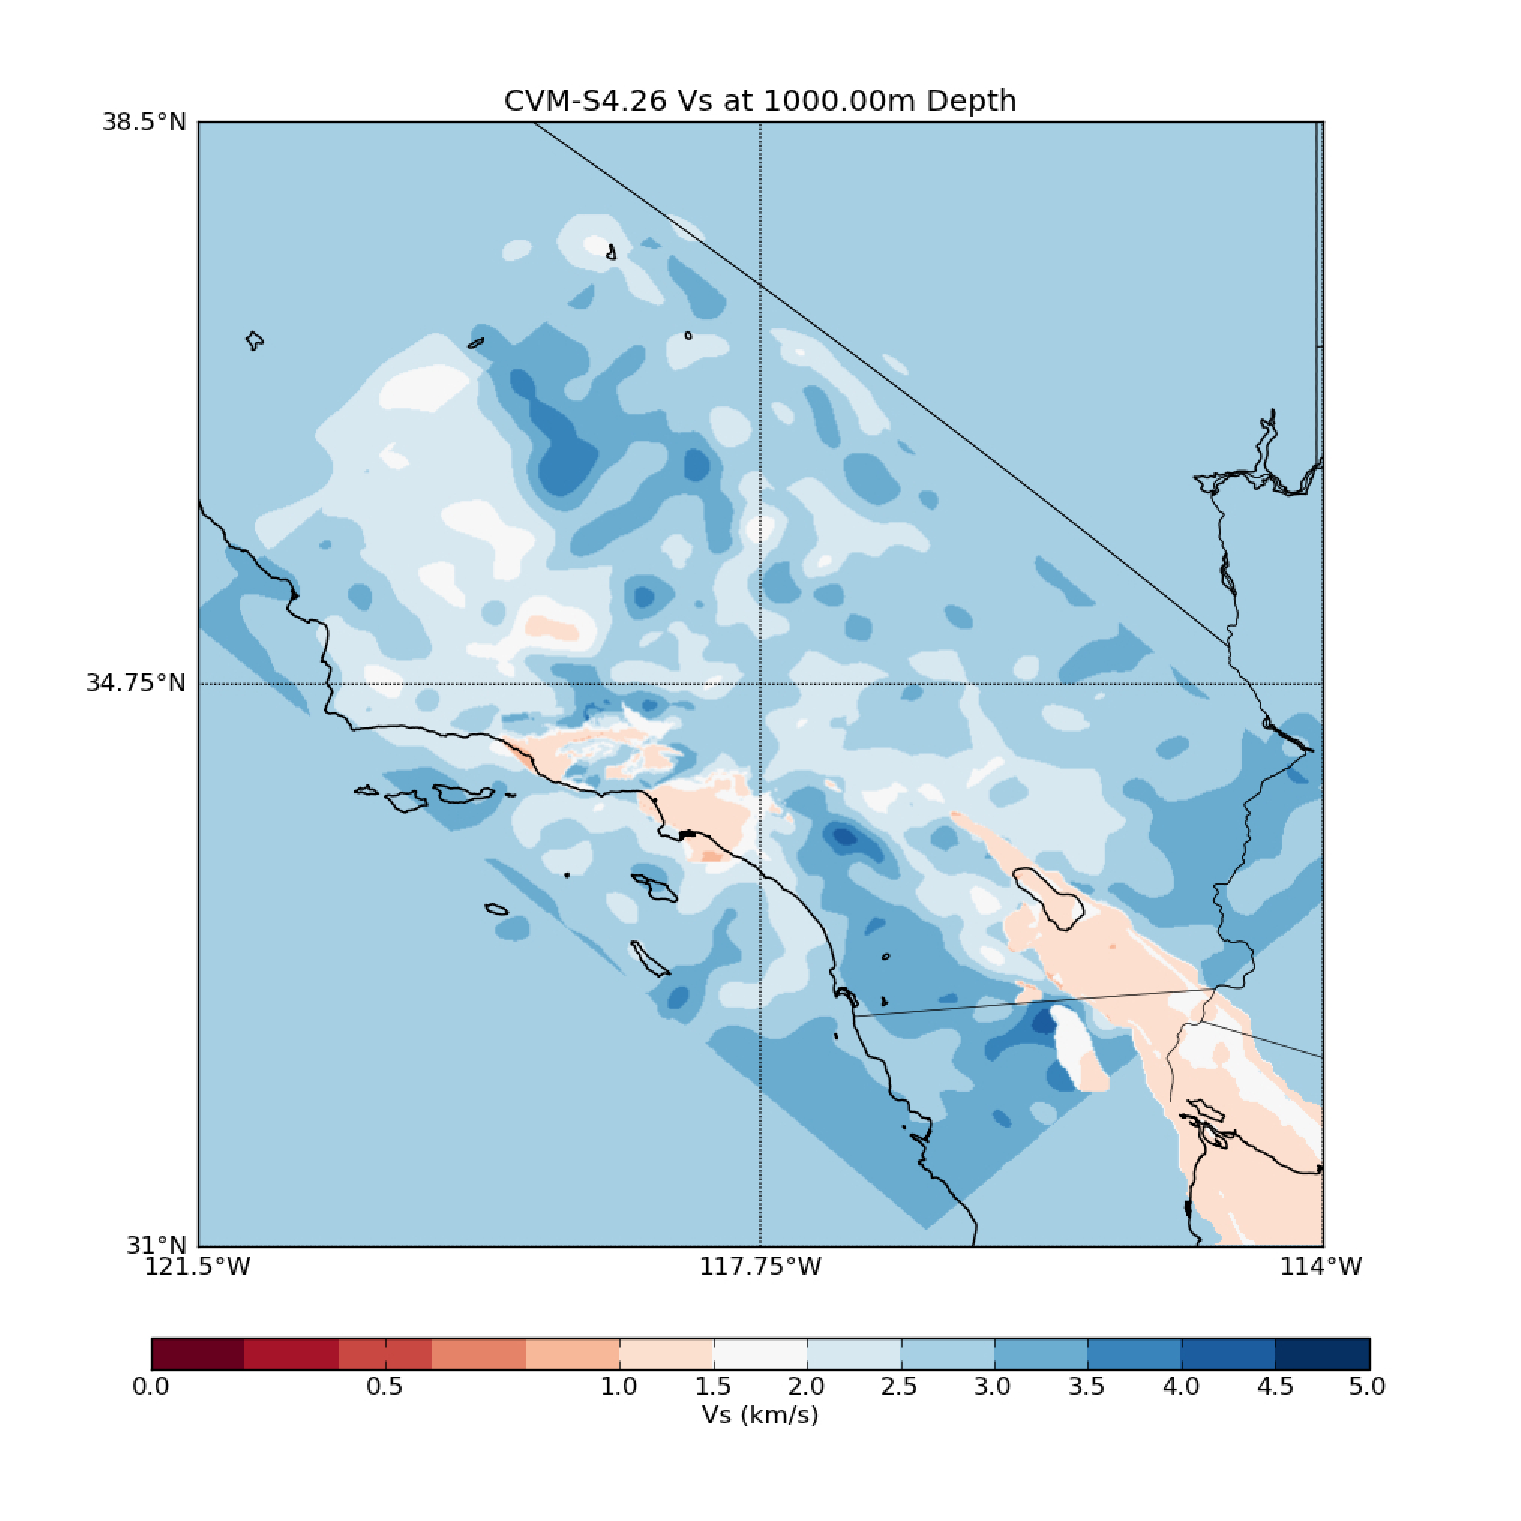
\includegraphics
                [width=0.5\textwidth]
                {figures/pdf/cvms426}

\textcolor{blue}{The map above was generated using the following inputs. User-entered text is denoted in red.}

\lstdefinestyle{cvms426-map-output}{
	moredelim=**[is][\color{red}]{@}{@}
}

\begin{lstlisting}[
        frame=none,
        basewidth={0.45em,0.4em},
        basicstyle=\ttfamily\footnotesize,breaklines=true,
        linewidth=0.98\columnwidth,xleftmargin=0.07\columnwidth,
        numbers=left,numberblanklines=true,numberstyle=\scriptsize\color{mylistingnclr},
	style=cvms426-map-output]
> ./horizontal_slice.py
> Plot Horizontal Slice - UCVM 14.3.0
>
> This utility helps you plot a horizontal slice across the earth for one of the CVMs
> that you installed with UCVM.
>
> In order to create the plot, you must first specify the region.
>
> Please enter the bottom-left longitude from which the plot should start: @-121.5@
> Next, enter the bottom-left latitude from which the plot should start: @31@
> Enter the top-right longitude where the plot should end: @-114@
> Enter the top-right latitude where the plot should end: @38.5@
> Which grid spacing (in decimal degree units) would you like (usually, this is 0.01): @0.01@
>
> Please enter the depth, in meters, at which you would like this plot: @1000@
>
> What would you like to plot (either vp, vs, rho, or poisson): @vs@
>
> From which CVM would you like this data to come:
>	1) CVM-S4
>	2) CVM-H 11.9.1
>	3) CVM-H 11.9.1 No GTL
>	4) CVM-S4.26
>	5) 1D
>	6) Broadband Whittier Narrows 1D Model
>	7) 1D w/ Vs30 GTL
>
> Select the CVM: @4@
>
> Finally, would you like a descritized or smooth color scale
> (enter 'd' for discrete, 's' for smooth): @d@
>
> Retrieving data. Please wait...
> Data retrieved successfully.
>
> Would you like to:
>	1) Save the data
>	2) Generate a plot
>
> Select one: @2@
\end{lstlisting}

\textcolor{blue}{All of the plotting scripts bundled with UCVM work in a very similar manner. Launching the script will ask a series of questions asking the user to define the region for the plot, the material property ($V_p$, $V_s$, or $\rho$) to plot, the model from which the data should come, and whether or not to save the data to an ASCII text file or display a graphical PNG image.} 
